\chapter{Use cases}

For illustrating the functionality of the aplication, we propose the following three use cases:

\section{First use case}

\begin{figure}[H]
	\centering
	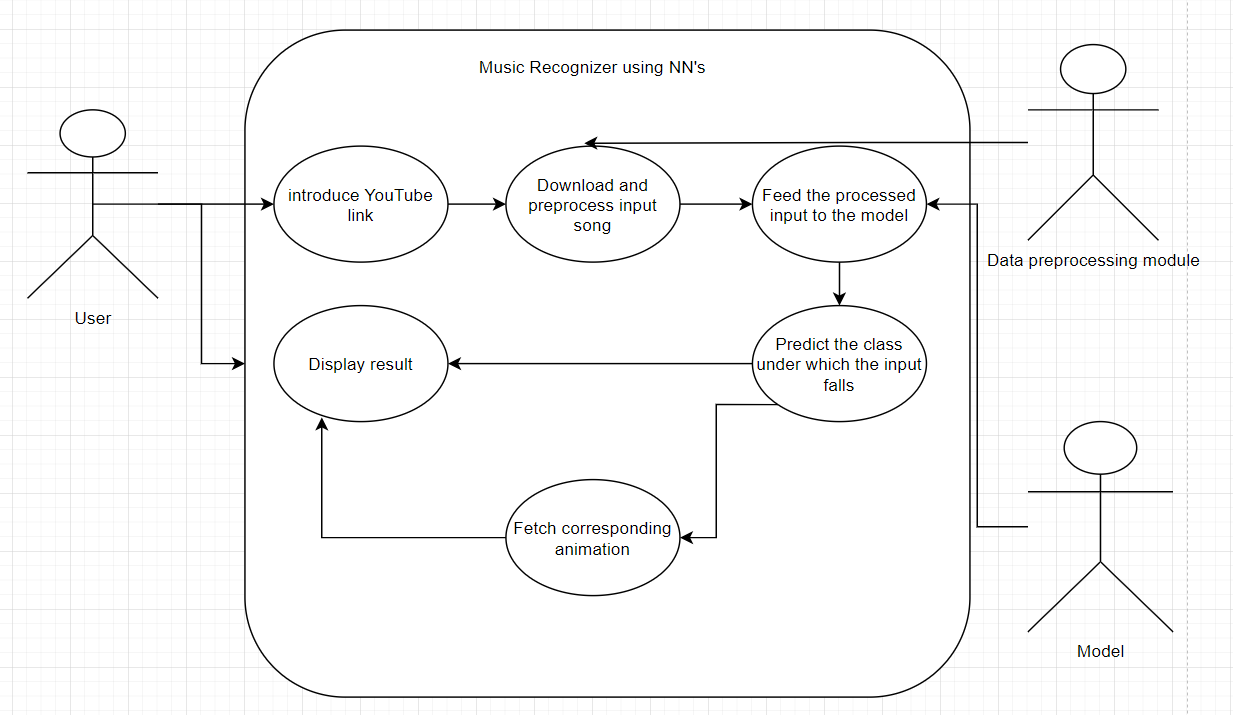
\includegraphics[width = 5.5in]{images/usecase1.png}
	\caption{Illustration of the application behaviour when the user inputs a correct link.}
	\label{uc1}
	\end{figure}
The application has the expected behaviour.
\section{Second use case}
\begin{figure}[H]
	\centering
	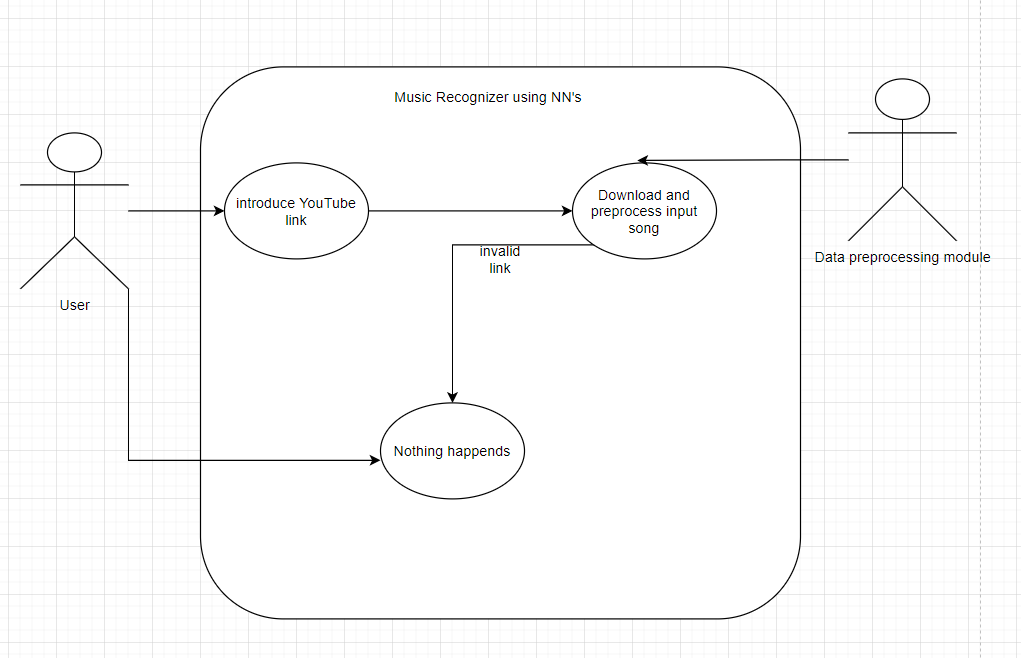
\includegraphics[width = 5.5in]{images/usecase3.png}
	\caption{Illustration of the application behaviour when the uses inputs an invalid link. }
	\label{uc3}
	\end{figure}
The link introduced by the user is invalid. The youtube-dl library will throw an exception and the execution will be ceased, given that the input cannot be fetched.

\section{Third use case}

\begin{figure}[H]
	\centering
	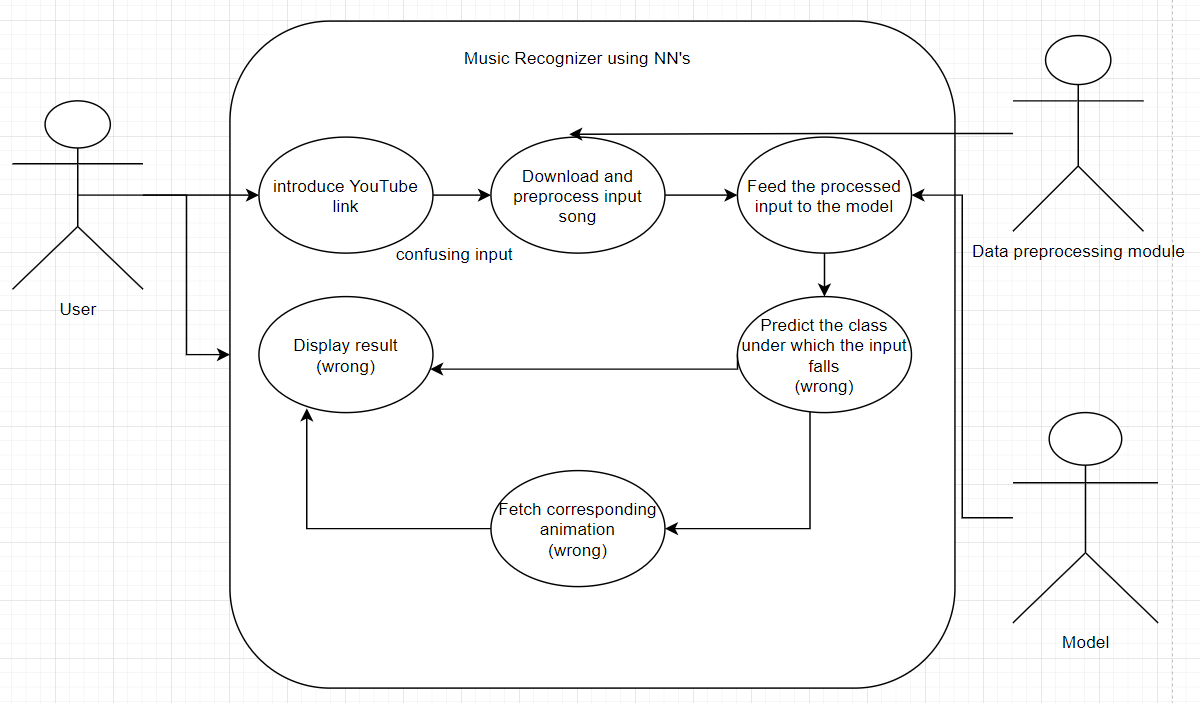
\includegraphics[width = 5.5in]{images/usecase2.png}
	\caption{Illustration of the application behaviour when the user inputs a confusing song to the application.}
	\label{uc2}
	\end{figure}
 The input is confusing (e.g. a symphonic concert containing multiple other instruments beside a piano). Given that the model has been trained on piano-only samples, the prediction for such an input will be 'Other'.
